\documentclass[a4paper]{article}
\usepackage[12pt]{extsizes}
\usepackage[utf8]{inputenc}
\usepackage[T2A]{fontenc}
\usepackage{amssymb,amsmath,mathtext}
\usepackage{indentfirst,amsfonts}
\usepackage[english, russian]{babel}
\usepackage{setspace,amsmath}
\usepackage{graphicx}
\usepackage[left=15mm, top=20mm, right=10mm, bottom=20mm, nohead, footskip=10mm]{geometry} % настройки полей документа

\graphicspath{{}}
\usepackage{minted}
\begin{document}
	\begin{titlepage} % начало документа
		
		% НАЧАЛО ТИТУЛЬНОГО ЛИСТА
		\begin{center}
			\footnotesize{ФЕДЕРАЛЬНОЕ ГОСУДАРСТВЕННОЕ БЮДЖЕТНОЕ ОБРАЗОВАТЕЛЬНОЕ }\\ 
			\footnotesize{УЧРЕЖДЕНИЕ ВЫСШЕГО ОБРАЗОВАНИЯ}\\
			\small{«МОСКОВСКИЙ ГОСУДАРСТВЕННЫЙ УНИВЕРСИТЕТ}\\
			\small{имени М.В.ЛОМОНОСОВА»}\\
			\hfill \break
			\normalsize{ФИЗИЧЕСКИЙ ФАКУЛЬТЕТ}\\
			\hfill \break
			\normalsize{КАФЕДРА МАТЕМАТИЧЕСКОГО МОДЕЛИРОВАНИЯ И ИНФОРМАТИКИ}\\
			\hfill \break
			\hfill \break
			\hfill \break
			\hfill \break
			\hfill \break
			\hfill \break
			\large{\textbf{Отчет по практическому заданию по численным методам}}\\
			\hfill \break
			\large{\textbf{Метод имитации отжига}}\\
		\end{center}
		
		\hfill \break
		
		\begin{flushright}
			Выполнил студент \\
			\hfill \break
			435 группы:\\
			\hfill \break
			Будакян Я. С.\\
			\hfill \break
			\hfill \break
			\hfill \break
		\end{flushright}
		
		\hfill \break
		\hfill \break
		\hfill \break
		\hfill \break
		\hfill \break
		\hfill \break
		
		\begin{center}
			Москва \\
			\hfill \break
			2017 
		\end{center}
		
		\thispagestyle{empty} % выключаем отображение номера для этой страницы
		
		% КОНЕЦ ТИТУЛЬНОГО ЛИСТА
		
	\end{titlepage}  % КОНЕЦ ДОКУМЕНТА !
	%учитываем титульный лист в нумерации
	\setcounter{page}{2}
	\section{Метод имитации отжига}
		\subsection{Описание}
			Метод имитации отжига - это метод стохастической оптимизации, использующий упорядоченный случайный поиск на основе аналогии с процессом образования в веществе кристаллической структуры при охлаждении. Преимуществом метода отжига являются возможность избегать локальных минимумов оптимизируемой функции за счет принятия временно ухудшающих результат решений, что отражает суть процесса нагрева расплава для предотвращения его быстрого остывания. Метод отжига отличается от итеративных алгоритмов адаптивностью. \\
			Метод отжига является одним из алгоритмов поиска глобального экстремума целевой функции $f(x)$, заданной для $x \in S$. Элементы множества $S$, дискретного или непрерывного, представляют собой состояния воображаемой физической системы("энергетические уровни"). Значение функции $f$ в этих точках используется как энергия системы $E = f(x)$. В каждый момент времени температура системы предполагается заданной. Находясь в состоянии с температурой $T$, следующее состояние системы выбирается в соответствии с заданным семейством вероятностных распределений $Q(x, T)$, которое задает новый случайный элемент $x^l = G(x, T)$. После генерации $x^l$ система с вероятностью $h(\Delta E; T)$ переходит к следующему шагу в следующее состояние $x^l$. Если этот переход не произошел, процесс генерации $x^l$ повторяется. Здесь $\Delta E$ обозначает приращение функции $f(x^l) - f(l)$. \\
			Конкретная схема отжига задается следующими параметрами:
			\begin{itemize}
				\item Выбором закона изменения температуры $T(k)$ на шаге $k$
				\item Выбором вероятностного распределения $Q(x; T)$
				\item Выбором функции вероятности принятия решения $h(\Delta E; T)$
			\end{itemize}
			В общем виде алгоритм можно представить в следующем виде:
			\begin{itemize}
				\item Случайным образом выбирается начальная точка $x = x_0; x_0 \in S$. Текущее значение энергии $E$ устанавливается равным $f(x_0)$.
				\item $k$-я итерация основного цикла состоит из шагов:
					\begin{itemize}		
						\item Сравнить энергию системы $E$ в состоянии $x$ с найденным на данный момент глобальным минимумом. Если $E = f(x)$ меньше, то изменить значение глобального минимума.
						\item Сгенерировать новую точку $x^l = G(x; T(k))$.
						\item Вычислить в ней значение $E^l = f(x^l)$.
						\item Сгенерировать случайное число $\alpha \sim U[0;1]$
						\item Если $\alpha < h(E^l - E; T(k))$, то:
							\begin{itemize}
								\item установить $x \longrightarrow x^l; E \longrightarrow E^l$
								\item Перейти к следующей итерации
							\end{itemize}
						\item Иначе, повторить процесс генерации
					\end{itemize}
			\end{itemize}
		\newpage
		\subsection{Реализация(Python)}
			\begin{minted}[linenos, autogobble]{python}
				# импортируем все необходимое
				import numpy as np
				import matplotlib.pyplot as plt
				import seaborn as sns
				%matplotlib inline
				# задаем функцию изменения температуры
				def decreaseTemperature(init_T, k, alpha):
					return init_T * alpha / k
				# задаем функцию вероятности принятия решения
				def transitProbability(dE, T):
					return np.exp(-dE / T)
				# функция принятия решения о переходе
				def isTransit(P):
					dec = np.random.rand()
					if (dec <= P):
						return True
					else:
						return False
				# функция генерации нового состояния
				def newState(left_bound, right_bound):
					return left_bound + (right_bound - left_bound) * np.random.rand()
				
				def simulatedAnnealing(energyFunc, left_bound, right_bound, init_T, end_T, alpha):
					# начальное состояние
					state = newState(left_bound, right_bound)
					T = init_T
					E = energyFunc(state)
					# количество итераций
					n = 0
					while (T > end_T):
						n += 1
						new_state = newState(left_bound, right_bound)
						new_E = energyFunc(new_state)
						if (new_E < E):
							E = new_E
							state = new_state
						else:
							P = transitProbability(new_E - E, T)
							if(isTransit(P)):
								E = new_E
								state = new_state
						T = decreaseTemperature(init_T, n, alpha)
					return (state, E)
			\end{minted}
		\newpage
		\section{Исследование}
			Проверим сначала реализацию на каком-нибудь простом примере, например, квадратичной функции $f(x) = 5x^2 + 6x - 4$:
			\begin{minted}[linenos, autogobble]{python}
				f = lambda x: 5 * x**2 + 6 * x - 4
				x = np.linspace(-5, 5, 50)
				y = f(x)
				plt.plot(x, y)
			\end{minted}
			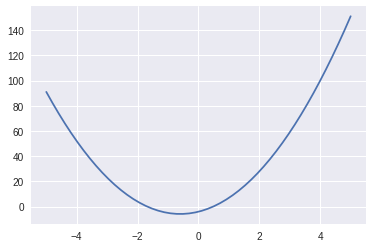
\includegraphics[width=0.5\linewidth]{parabola}
			\begin{minted}[linenos, autogobble]{python}
				x_min, f_min = simulatedAnnealing(f, -5, 5, 10, 0.001, 0.1)
				print('Minimum found: state = {}, E = {}'.format(x_min, f_min))
				
				Minimum found: state = -0.5957411989856904, E = -5.799909313069603
			\end{minted}
			Аналитический минимум: $x_{min} = -\frac{3}{5}$, $f(x_{min}) = -\frac{29}{5} $, что с хорошей точностью совпадает с полученным отжигом результатом. \\
			Исследуем поведение отжига на более сложной функции:
			\begin{minted}[linenos, autogobble]{python}
				# значение функции задано набором точек
				Y = np.load('earr.npy')
				fig = plt.figure(figsize=(12,4))
				plt.plot(Y)
			\end{minted}
			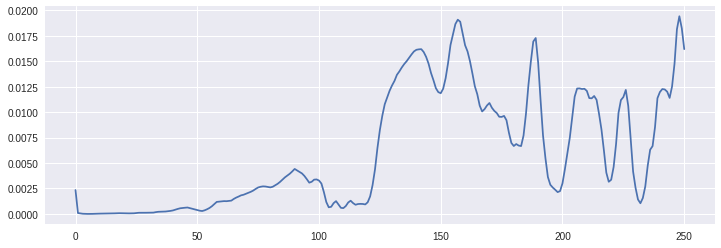
\includegraphics[width=\linewidth]{earr-1}
			\newpage
			\begin{minted}[linenos, autogobble]{python}
				def F(x):
					index = int(x)
					return Y[index]
			\end{minted}
			Переберем несколько наборов параметров:
			\begin{itemize}
				\item $T_0 = [100, 10, 1]$
				\item $T_f = [0.01, 0.001, 0.0001, 0.00001]$
				\item $\alpha = [1, 0.1, 0.01]$
			\end{itemize}
			\begin{minted}[linenos, autogobble]{python}
				x_mins = np.zeros((3, 4, 3))
				F_mins = np.zeros((3, 4, 3))
				for i, init_T in enumerate([100, 10, 1]):
					for j, end_T in enumerate([0.01, 0.001, 0.0001, 0.00001]):
						for k, alpha in enumerate([1, 0.1, 0.01]):
							x_min, F_min = simulatedAnnealing(F, 0, 251,
											init_T, end_T, alpha)
							x_mins[i, j, k] = x_min
							F_mins[i, j, k] = F_min
			\end{minted}
			Отобразим полученные результаты на графике функции:
			\begin{minted}[linenos, autogobble]{python}
				fig = plt.figure(figsize=(12,4))
				plt.plot(Y)
				plt.plot(list(map(int, x_mins.ravel())), Y[list(map(int, x_mins.ravel()))], 'ro')
			\end{minted}
			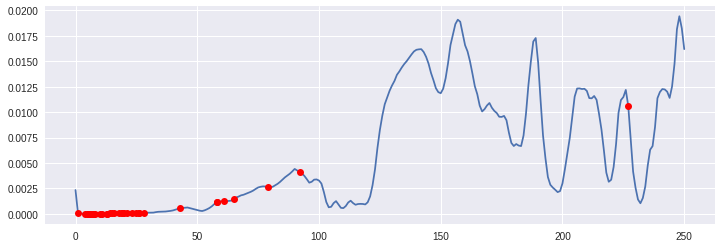
\includegraphics[width=\linewidth]{earr-2}
			Посмотрим на отдельные зависимости:
			\begin{minted}[linenos, autogobble]{python}
				fig = plt.figure(figsize=(12,4))
				plt.plot(Y)
				plt.plot(list(map(int, x_mins[:, 3, 2])), Y[list(map(int, x_mins[:, 3, 2]))], 'ro')
				plt.plot(list(map(int, x_mins[2, :, 2])), Y[list(map(int, x_mins[2, :, 2]))], 'bo')
				plt.plot(list(map(int, x_mins[2, 3, :])), Y[list(map(int, x_mins[2, 3, :]))], 'go')
			\end{minted}
			\newpage
			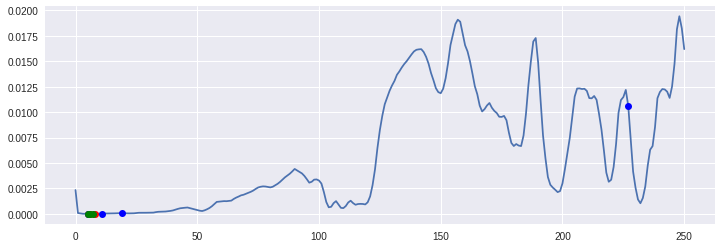
\includegraphics[width=\linewidth]{earr-3}
			Видно, что качество найденного решения сильно зависит от конечной температуры, и слабо - от начальной и коэффициента альфа(они влияют на время выполнения, т.к. от них зависит итоговое количество итераций).
\end{document}